% ════════════════════════════════════════════════════════════════════════════
% content/chapters/chapter2.tex
% ════════════════════════════════════════════════════════════════════════════

\chapter{Hito 2: Los datos -- origen, descripci\'on y an\'alisis}

% ─────────────────────────────────────────────────────────────────────────────
\section{Introducci\'on al Hito 2}

En este hito se describen y analizan los datos disponibles para abordar el problema
planteado en el Hito anterior: diseñar, implementar y validar un sistema inteligente capaz
de \textbf{clasificar la variedad vinícola de un vino} a partir de sus propiedades
fisicoqu\'imicas, con el objetivo de apoyar al en\'ologo en la toma de decisiones de
calidad de forma objetiva y reproducible.

El an\'alisis que se describe tiene como objetivo comprender los datos, detectar
posibles sesgos y limitaciones, y evaluar en qu\'e medida el conjunto de datos
disponible permite abordar el problema planteado.

% ─────────────────────────────────────────────────────────────────────────────
\section{Fuentes, origen y tama\~no}

La fuente de datos seleccionada es el \textbf{Wine Recognition Dataset}, disponible
en el repositorio UCI Machine Learning Repository \cite{UCIWine}. Este dataset recoge
los resultados de an\'alisis qu\'imicos realizados sobre vinos producidos en la misma
regi\'on de Italia, pero procedentes de \textbf{tres cultivares distintos}.

\subsection{Justificaci\'on de la fuente de datos}

La elecci\'on de este dataset se debe a los siguientes motivos:

\begin{itemize}
    \item \textbf{Relevancia para el dominio:} Las 13 variables fisicoqu\'imicas
    (alcohol, acidez, fenoles, etc.) son las magnitudes que los laboratorios
    vitivin\'icolas miden de forma rutinaria para la certificaci\'on de calidad y
    variedad.
    \item \textbf{Variables bien definidas:} Cada columna tiene una interpretaci\'on
    clara desde la perspectiva enol\'ogica, esto facilita la validaci\'on con el
    experto en dominio.
    \item \textbf{Disponibilidad y reproducibilidad:} Al ser un dataset p\'ublico y
    ampliamente utilizado, permite comparar los resultados del sistema con benchmarks 
    establecidos.
    \item \textbf{Ausencia de valores faltantes:} El dataset est\'a completo, lo que
    elimina la necesidad de estrategias de imputaci\'on que pudieran introducir sesgos
    adicionales.
\end{itemize}

\subsection{Estructura y tama\~no del dataset}

El dataset presenta las siguientes caracter\'isticas generales:

\begin{table}[H]
    \centering
    \caption{Caracter\'isticas generales del dataset Wine UCI}
    \begin{tabular}{ll}
        \toprule
        \textbf{Caracter\'istica}        & \textbf{Valor}                            \\
        \midrule
        N\'umero de instancias (filas)   & 178                                       \\
        N\'umero de variables (columnas) & 13 + 1 variable objetivo                 \\
        Valores faltantes                & 0 (dataset completo)                      \\
        Tipo de problema                 & Clasificaci\'on multiclase supervisada    \\
        N\'umero de clases               & 3 (cultivares de vino)                    \\
        Tipo de datos                    & Num\'erico continuo (todas las variables) \\
        Formato                          & CSV (.csv)                                \\
        \bottomrule
    \end{tabular}
    \label{tab:general}
\end{table}

La distribuci\'on de instancias por clase es la siguiente:

\begin{table}[H]
    \centering
    \caption{Distribuci\'on de clases en el dataset}
    \begin{tabular}{cccc}
        \toprule
        \textbf{Clase} & \textbf{Cultivar} & \textbf{N.\textordmasculine{} muestras} & \textbf{\%} \\
        \midrule
        1              & Cultivar 1        & 59   & 33.1\% \\
        2              & Cultivar 2        & 71   & 39.9\% \\
        3              & Cultivar 3        & 48   & 27.0\% \\
        \midrule
        \textbf{Total} & --                & \textbf{178} & \textbf{100\%} \\
        \bottomrule
    \end{tabular}
    \label{tab:clases}
\end{table}

\vspace{0.5cm}

Desde el punto de vista del volumen, nos encontramos ante un problema de
\textbf{small data} (178 instancias). Dado el reducido número de instancias, el uso de modelos con alta capacidad expresiva debe controlarse mediante validación cruzada estratificada para evitar sobreajuste.

\vspace{1.5mm}

Adicionalmente, la distribución de clases no es perfectamente uniforme (27\%–40\%), por lo que nos encontramos con una distribución de clases levemente desbalanceada, pero no es extrema ni problemática. A pesar de no ser un requisito indispensable dado el bajo desbalanceo, se utilizarán métricas que no sean sensibles a la disparidad de clases (F1-Macro o Precisión Balanceada) para asegurar un rendimiento equilibrado entre los diferentes tipos de vino. 

% ─────────────────────────────────────────────────────────────────────────────
\section{Inventario de datos}

En esta secci\'on se detalla el diccionario de variables del dataset. Este inventario
ha sido elaborado con el apoyo del experto en dominio del equipo (Antonio Mu\~noz
Garc\'ia), quien ha validado la relevancia enol\'ogica de cada variable con respecto
al problema de clasificaci\'on de cultivares.

% Tabla dividida en dos partes para evitar desbordamiento de página
\begin{table}[H]
    \centering
    \caption{Inventario de datos -- Diccionario de variables (parte 1/2)}
    \small
    \begin{tabular}{p{4cm} p{6.5cm} p{1.8cm} p{1.5cm}}
        \toprule
        \textbf{Variable} & \textbf{Descripci\'on} & \textbf{Tipo} & \textbf{Unidad} \\
        \midrule
        \texttt{Alcohol}
            & Contenido alcoh\'olico del vino
            & Num. cont. & \% vol \\[3pt]
        \texttt{MalicAcid}
            & Concentraci\'on de \'acido m\'alico
            & Num. cont. & g/L \\[3pt]
        \texttt{Ash}
            & Contenido en cenizas (minerales totales)
            & Num. cont. & g/L \\[3pt]
        \texttt{AlcalinityAsh}
            & Alcalinidad de las cenizas
            & Num. cont. & mEq/L \\[3pt]
        \texttt{Magnesium}
            & Concentraci\'on de magnesio
            & Num. cont. & mg/L \\[3pt]
        \texttt{TotalPhenols}
            & Contenido total de fenoles
            & Num. cont. & g/L \\[3pt]
        \texttt{Flavanoids}
            & Contenido de flavanoides
            & Num. cont. & g/L \\
        \bottomrule
    \end{tabular}
    \label{tab:diccionario1}
\end{table}

\begin{table}[H]
    \centering
    \caption{Inventario de datos -- Diccionario de variables (parte 2/2)}
    \small
    \begin{tabular}{p{4cm} p{6.5cm} p{1.8cm} p{1.5cm}}
        \toprule
        \textbf{Variable} & \textbf{Descripci\'on} & \textbf{Tipo} & \textbf{Unidad} \\
        \midrule
        \texttt{NonflavanoidPhenols}
            & Fenoles no flavanoides
            & Num. cont. & g/L \\[3pt]
        \texttt{Proanthocyanins}
            & Contenido de proantocianidinas
            & Num. cont. & g/L \\[3pt]
        \texttt{ColorIntensity}
            & Intensidad del color del vino
            & Num. cont. & u.a. \\[3pt]
        \texttt{Hue}
            & Tonalidad del vino
            & Num. cont. & u.a. \\[3pt]
        \texttt{OD280/OD315}
            & Relaci\'on de absorbancias (calidad prote\'inas)
            & Num. cont. & u.a. \\[3pt]
        \texttt{Proline}
            & Concentraci\'on del amino\'acido prolina
            & Num. cont. & mg/L \\[3pt]
        \midrule
        \texttt{Class}
            & Clase de cultivar (1, 2 o 3) --
              \textbf{variable objetivo}
            & Categ\'orica & -- \\
        \bottomrule
    \end{tabular}
    \label{tab:diccionario2}
\end{table}

Todas las variables de entrada son num\'ericas continuas, lo que simplifica
el preprocesado. Sin embargo, la diversidad de escalas (e.g., \texttt{Proline} oscila
entre 278 y 1680~mg/L mientras que \texttt{Hue} toma valores entre 0.48 u.a. y 1.71 u.a. ) hace
imprescindible aplicar una \textbf{normalizaci\'on} antes del
entrenamiento de modelos sensibles a la escala de los datos.

% ─────────────────────────────────────────────────────────────────────────────
\section{An\'alisis de los datos}

El análisis exploratorio de los datos se ha realizado mediante un cuaderno
de R desarrollado específicamente para este hito~\cite{eda_script}, cuyo
código está disponible en el repositorio VinOps~\cite{vinops_repo}.

\begin{enumerate}
    \item Estad\'isticos descriptivos de todas las variables.
    \item An\'alisis estadístico por clase.
    \item Análisis de distribuciones por clase.
    \item An\'alisis de correlaciones entre variables.
    \item An\'alisis de componentes principales (PCA).
    \item Detecci\'on de valores at\'ipicos mediante PCA
    \item Exploración de los datos usando PCA
\end{enumerate}

\subsection{Estad\'isticos descriptivos}

La Tabla~\ref{tab:estadisticos} resume los principales estad\'isticos descriptivos
del dataset.

\begin{table}[H]
    \centering
    \caption{Estad\'isticos descriptivos del dataset}
    \small
    \begin{tabular}{lrrrrrr}
        \toprule
        \textbf{Variable}       & \textbf{M\'in} & \textbf{Q1} & \textbf{Med.}
                                & \textbf{Media} & \textbf{Q3} & \textbf{M\'ax} \\
        \midrule
        Alcohol             & 11.03 & 12.36 & 13.05 & 13.00 & 13.68 & 14.83 \\
        MalicAcid           & 0.74  & 1.60  & 1.87  & 2.34  & 3.08  & 5.80  \\
        Ash                 & 1.36  & 2.21  & 2.36  & 2.37  & 2.56  & 3.23  \\
        AlcalinityAsh       & 10.6  & 17.2  & 19.5  & 19.5  & 21.5  & 30.0  \\
        Magnesium           & 70    & 88    & 98    & 99.7  & 107   & 162   \\
        TotalPhenols        & 0.98  & 1.74  & 2.35  & 2.29  & 2.80  & 3.88  \\
        Flavanoids          & 0.34  & 1.21  & 2.13  & 2.03  & 2.88  & 5.08  \\
        NonflavanoidPhenols & 0.13  & 0.27  & 0.34  & 0.36  & 0.44  & 0.66  \\
        Proanthocyanins     & 0.41  & 1.25  & 1.55  & 1.59  & 1.95  & 3.58  \\
        ColorIntensity      & 1.28  & 3.22  & 4.69  & 5.06  & 6.20  & 13.00 \\
        Hue                 & 0.48  & 0.78  & 0.96  & 0.96  & 1.12  & 1.71  \\
        OD280/OD315         & 1.27  & 1.94  & 2.78  & 2.61  & 3.17  & 4.00  \\
        Proline             & 278   & 500   & 673   & 747   & 985   & 1680  \\
        \bottomrule
    \end{tabular}
    \label{tab:estadisticos}
\end{table}

De la inspecci\'on de estos estad\'isticos se extraen las siguientes observaciones:

\begin{itemize}
    \item \textbf{Diversidad de escalas:} La variable \texttt{Proline} presenta
    valores hasta 1680~mg/L, mientras que \texttt{Hue} oscila entre 0.48 y 1.71.
    Esta heterogeneidad hace imprescindible la normalizaci\'on antes del entrenamiento
    de modelos basados en distancias o gradientes.

    \item \textbf{Distribuciones asim\'etricas:} \texttt{MalicAcid} presenta una
    media (2.34) notablemente superior a su mediana (1.87), indicando sesgo positivo.
    Lo mismo ocurre con \texttt{ColorIntensity} y \texttt{Proline}. Estas asimetr\'ias
    pueden impactar en modelos que asumen normalidad.

    \item \textbf{Variables con baja variabilidad relativa:} \texttt{Ash} y
    \texttt{NonflavanoidPhenols} presentan rangos intercuart\'ilicos reducidos, lo
    que sugiere que tal vez no puedan aportar tan información por sí solas.
\end{itemize}

\subsection{An\'alisis estadístico por clase}


Para cuantificar de forma descriptiva el grado de separación entre clases en cada variable,
se empleó la siguiente medida de diferencia relativa entre medias:

\[
\Delta_{\text{rel}} = 
\frac{\max(\bar{x}_k) - \min(\bar{x}_k)}
{\displaystyle \frac{1}{K} \sum_{k=1}^{K} \bar{x}_k}
\]

donde:

\begin{itemize}
    \item $\bar{x}_k$ es la media de la variable en la clase $k$,
    \item $K$ es el número de clases (en nuestro caso, $K = 3$).
\end{itemize}

Esta medida calcula el rango máximo entre medias de clase y lo normaliza
dividiéndolo por la media global de dichas medias, obteniendo una cantidad global que permite determinar la diferenciación entre las clases.
\begin{table}[H]
\centering
\caption{Medias por clase y diferencia relativa entre clases}
\begin{tabular}{lccccc}
\toprule
\textbf{Variable} & \textbf{Clase 1} & \textbf{Clase 2} & \textbf{Clase 3} & $\boldsymbol{\Delta_{rel}}$ & \textbf{Nivel} \\
\midrule
\texttt{Flavanoids}              & 2.98   & 2.08   & 0.78   & 1.13 & \textbf{Muy alta} \\
\texttt{Color\_Intensity}        & 5.53   & 3.09   & 7.40   & 0.81 & \textbf{Muy alta} \\
\texttt{Proline}                 & 1115.71& 519.51 & 629.90 & 0.79 & \textbf{Muy alta} \\
\texttt{OD280\_OD315}            & 3.16   & 2.79   & 1.68   & 0.58 & \textbf{Alta} \\
\texttt{Malic\_Acid}             & 2.01   & 1.93   & 3.33   & 0.58 & \textbf{Alta} \\
\texttt{Total\_Phenols}          & 2.84   & 2.26   & 1.68   & 0.51 & \textbf{Alta} \\
\texttt{Proanthocyanins}         & 1.90   & 1.63   & 1.15   & 0.48 & Moderada \\
\texttt{Nonflavanoid\_Phenols}   & 0.29   & 0.36   & 0.45   & 0.43 & Moderada \\
\texttt{Hue}                     & 1.06   & 1.06   & 0.68   & 0.41 & Moderada \\
\texttt{Alcalinity\_of\_Ash}     & 17.04  & 20.24  & 21.42  & 0.22 & Bajo \\
\texttt{Magnesium}               & 106.34 & 94.55  & 99.31  & 0.12 & Bajo \\
\texttt{Alcohol}                 & 13.74  & 12.28  & 13.15  & 0.11 & Bajo \\
\texttt{Ash}                     & 2.46   & 2.24   & 2.44   & 0.09 & Bajo \\
\bottomrule
\end{tabular}
\label{tab:medias_clase_diff}
\end{table}

De este análisis descriptivo se observa que:

\begin{itemize}

    \item \textbf{\texttt{Flavanoids}}, \textbf{\texttt{Color\_Intensity}} y 
    \textbf{\texttt{Proline}} presentan las mayores diferencias relativas entre
    medias de clase, lo que indica una mayor diferenciación entre cultivares
    en términos de valores medios.

    \item En contraste, variables como \textbf{\texttt{Ash}},
    \textbf{\texttt{Alcohol}}, \textbf{\texttt{Magnesium}} y
    \textbf{\texttt{Alcalinity\_of\_Ash}} muestran medias más similares entre
    clases.

    \item La \textbf{Clase 3} destaca por un perfil medio claramente diferenciado
    en varias variables, especialmente por sus valores bajos en
    \texttt{Flavanoids} y altos en \texttt{Color\_Intensity} y
    \texttt{Malic\_Acid}.

    \item Las \textbf{Clases 1 y 2} presentan medias más próximas en varias
    variables, lo que podría hacer más compleja su separación si se consideran
    únicamente diferencias de promedio.

\end{itemize}

Cabe señalar que esta medida describe únicamente diferencias entre medias y
no tiene en cuenta la dispersión dentro de cada clase, por lo que sus resultados
deben interpretarse como un análisis preliminar.

\subsection{Análisis de distribuciones univariantes}

El análisis de los histogramas generados para cada variable permite caracterizar
la forma, dispersión y posibles valores extremos presentes en el dataset. Este
estudio descriptivo constituye una etapa previa al análisis detallado
y no implica, por sí mismo, conclusiones sobre capacidad discriminante.

\begin{itemize}

    \item \textbf{\texttt{Flavanoids}:} La distribución global presenta una
    estructura compatible con bimodalidad, con concentraciones de valores
    aproximadamente en los intervalos 0.5--1.0~g/L y 2.5--3.0~g/L.
    Esta configuración sugiere la posible existencia de subgrupos diferenciados
    en la muestra. No obstante, la interpretación en términos de separación entre
    clases requiere un análisis más profundo. 

    \item \textbf{\texttt{Proline}:} Variable con marcada asimetría positiva y
    amplio rango de valores (hasta 1680~mg/L). La presencia de cola larga y
    valores extremos indica alta variabilidad y posible influencia de outliers.
    Dada su escala significativamente mayor respecto a otras variables,
    resulta imprescindible considerar estandarización previa al modelado.

    \item \textbf{\texttt{MalicAcid}:} Distribución asimétrica hacia la derecha,
    con presencia de valores elevados en la cola superior. Esta estructura
    sugiere heterogeneidad en los niveles de acidez málica dentro de la muestra.

    \item \textbf{\texttt{ColorIntensity}:} Presenta cola larga hacia la derecha,
    con valores superiores a 10 que podrían considerarse extremos en términos
    descriptivos. La dispersión observada indica variabilidad relevante en esta
    característica físico-química.

    \item \textbf{\texttt{Ash}, \texttt{AlcalinityAsh}, \texttt{Magnesium}:}
    Distribuciones aproximadamente simétricas y concentradas en torno a sus
    valores centrales, con menor dispersión relativa en comparación con
    variables como \texttt{Proline} o \texttt{ColorIntensity}.

\end{itemize}

En conjunto, el análisis univariante revela que:

\begin{itemize}
    \item Existen diferencias notables en escala entre variables.
    \item Varias características presentan asimetría y posibles valores extremos.
    \item La heterogeneidad observada sugiere la conveniencia de aplicar
    técnicas de normalización o estandarización antes del entrenamiento de modelos.
\end{itemize}

Cabe destacar que estas observaciones describen únicamente el comportamiento
marginal de cada variable ($P(X)$). La evaluación de su capacidad para diferenciar
entre cultivares requiere el análisis de las distribuciones condicionadas por clase
($P(X \mid \text{Clase})$).


\subsection{Análisis de correlaciones}

El heatmap de correlaciones de Pearson muestra la existencia de relaciones
lineales relevantes entre varias variables físico-químicas. Las correlaciones
de mayor magnitud (|r| $\geq$ 0.50) se resumen a continuación:

\begin{table}[H]
\centering
\caption{Correlaciones relevantes entre variables del dataset}
\begin{tabular}{lcc}
\toprule
\textbf{Par de variables} & \textbf{r} & \textbf{Interpretación} \\
\midrule
\texttt{TotalPhenols} -- \texttt{Flavanoids}        & 0.86 & Muy alta positiva \\
\texttt{Flavanoids} -- \texttt{OD280\_OD315}        & 0.79 & Alta positiva \\
\texttt{TotalPhenols} -- \texttt{OD280\_OD315}      & 0.70 & Alta positiva \\
\texttt{Flavanoids} -- \texttt{Proanthocyanins}     & 0.65 & Moderada-alta positiva \\
\texttt{Alcohol} -- \texttt{Proline}                & 0.64 & Moderada-alta positiva \\
\texttt{TotalPhenols} -- \texttt{Color\_Intensity}  & 0.61 & Moderada positiva \\
\texttt{Hue} -- \texttt{OD280\_OD315}               & 0.57 & Moderada positiva \\
\texttt{Malic\_Acid} -- \texttt{Hue}                & -0.56 & Moderada negativa \\
\texttt{Flavanoids} -- \texttt{Nonflavanoid\_Phenols} & -0.54 & Moderada negativa \\
\texttt{Color\_Intensity} -- \texttt{Hue}           & -0.52 & Moderada negativa \\
\bottomrule
\end{tabular}
\label{tab:correlaciones}
\end{table}

\vspace{0.5cm}

Se observa un bloque claramente correlacionado formado por 
\texttt{TotalPhenols}, \texttt{Flavanoids} y \texttt{OD280\_OD315}, 
con coeficientes elevados y consistentes. Esta estructura sugiere que 
estas variables capturan información química parcialmente solapada, 
posiblemente asociada al contenido fenólico del vino. En términos 
estadísticos, ello indica la existencia de redundancia informativa y 
cierto grado de multicolinealidad entre estas características.

Asimismo, \texttt{Proanthocyanins} y \texttt{Color\_Intensity} muestran 
asociaciones relevantes con este grupo, lo que refuerza la idea de que 
existe un conjunto de variables relacionadas entre sí que describen 
propiedades químicas conectadas. 

\vspace{1.5mm}

Estas relaciones indican la presencia de estructura lineal interna en
el dataset y podrían justificar la exploración de técnicas de reducción
dimensional en la siguiente sección.

\subsection{An\'alisis de Componentes Principales (PCA)}

Se ha aplicado PCA sobre el dataset (con variables estandarizadas) para obtener una
representaci\'on de baja dimensionalidad que permita visualizar estructura y posibles agrupamientos por clase.

\begin{table}[H]
    \centering
    \caption{Varianza explicada por las primeras componentes principales}
    \begin{tabular}{ccc}
        \toprule
        \textbf{Componente} & \textbf{Varianza explicada} & \textbf{Varianza acumulada} \\
        \midrule
        PC1 & 36.2\% & 36.2\% \\
        PC2 & 19.2\% & 55.4\% \\
        PC3 & 11.12\% &   66.52\% \\
        PC4 &  7.07\% & 73.6\% \\
        PC5 &  6.57\% & 80.15 \% \\
        \bottomrule
    \end{tabular}
    \label{tab:pca}
\end{table}

Las conclusiones del análisis PCA son:

\begin{itemize}

    \item En el plano PC1--PC2 se observa una estructura agrupada por clases,
    con una diferenciación apreciable entre los tres cultivares. No obstante,
    existe cierto solapamiento, especialmente en la región ocupada por la
    Clase 2, por lo que no puede afirmarse una separabilidad perfecta en esta
    proyección bidimensional.

    \item \textbf{PC1} está fuertemente influida por variables relacionadas con
    el contenido fenólico (\texttt{Flavanoids}, \texttt{TotalPhenols},
    \texttt{OD280/OD315}), lo que sugiere que esta componente recoge un eje
    asociado a la riqueza polifenólica del vino.

    \item \textbf{PC2} está principalmente determinada por
    \texttt{ColorIntensity}, \texttt{MalicAcid} y \texttt{Proline}, aportando
    una segunda dimensión relevante de variabilidad química.

    \item Las dos primeras componentes explican el 58.4\% de la varianza total,
    lo que permite una representación visual informativa, aunque parte de la
    estructura del dataset permanece en componentes posteriores, pudiendo llegar al 75\% de la varianza utilizando dos componentes principales más.

\end{itemize}



\subsection{Detecci\'on de valores at\'ipicos}

Se han aplicado dos t\'ecnicas complementarias:

\begin{enumerate}
    \item \textbf{An\'alisis univariante (boxplot IQR):} Se identifican valores fuera
    del rango $[Q1 - 1.5 \cdot \mathrm{IQR},\; Q3 + 1.5 \cdot \mathrm{IQR}]$ para
    cada variable.

    \item \textbf{An\'alisis multivariante ($T^2$ de Hotelling y Q-residuals/SPE):}
    Implementado sobre el espacio PCA para detectar observaciones an\'omalas en el
    espacio multidimensional reducido.
\end{enumerate}

\begin{table}[H]
    \centering
    \caption{Outliers detectados mediante $T^2$ de Hotelling}
    \begin{tabular}{cc}
        \toprule
        \textbf{Observaci\'on}  & \textbf{Nivel de anomal\'ia} \\
        \midrule
        26, 61, 74, 124        & Moderado (entre $F_{95}$ y $F_{99}$) \\
        60, 70, 96, 97, 111, 122, 125 & Extremo (por encima de $F_{99}$) \\
        \bottomrule
    \end{tabular}
    \label{tab:outliers}
\end{table}

\begin{table}[H]
    \centering
    \caption{Outliers detectados mediante distancia al modelo (Q-residuals / SPE)}
    \begin{tabular}{cc}
        \toprule
        \textbf{Observaci\'on}  & \textbf{Nivel de anomal\'ia} \\
        \midrule
        72, 79, 100, 111, 122 & Moderado (entre $Q_{95}$ y $Q_{99}$) \\
        96, 159, 160          & Extremo (por encima de $Q_{99}$) \\
        \bottomrule
    \end{tabular}
    \label{tab:outliers_spe}
\end{table}

\noindent Estas observaciones ser\'an revisadas junto con el experto en dominio para
determinar si corresponden a errores de medici\'on en laboratorio o a vinos
genuinamente at\'ipicos. La decisi\'on de eliminarlos o mantenerlos se tomar\'a en
el hito de preprocesado.

\subsection{Exploración de los datos usando PCA}

\begin{table}[H]
\centering
\caption{Loadings de las variables en las cinco primeras componentes principales}
\begin{tabular}{lccccc}
\toprule
\textbf{Variable} & \textbf{Dim.1} & \textbf{Dim.2} & \textbf{Dim.3} & \textbf{Dim.4} & \textbf{Dim.5} \\
\midrule
Alcohol                & 0.1443 & 0.4837 & -0.2074 & -0.0179 & 0.2657 \\
Malic\_Acid            & -0.2452 & 0.2249 & 0.0890 & 0.5369 & -0.0352 \\
Ash                    & -0.0021 & 0.3161 & 0.6262 & -0.2142 & 0.1430 \\
Alcalinity\_of\_Ash    & -0.2393 & -0.0106 & 0.6121 & 0.0609 & -0.0661 \\
Magnesium              & 0.1420 & 0.2996 & 0.1308 & -0.3518 & -0.7270 \\
Total\_Phenols         & 0.3947 & 0.0650 & 0.1462 & 0.1981 & 0.1493 \\
Flavanoids             & 0.4229 & -0.0034 & 0.1507 & 0.1523 & 0.1090 \\
Nonflavanoid\_Phenols  & -0.2985 & 0.0288 & 0.1704 & -0.2033 & 0.5007 \\
Proanthocyanins        & 0.3134 & 0.0393 & 0.1495 & 0.3991 & -0.1369 \\
Color\_Intensity       & -0.0886 & 0.5300 & -0.1373 & 0.0659 & 0.0764 \\
Hue                    & 0.2967 & -0.2792 & 0.0852 & -0.4278 & 0.1736 \\
OD280\_OD315           & 0.3762 & -0.1645 & 0.1660 & 0.1841 & 0.1012 \\
Proline                & 0.2868 & 0.3649 & -0.1267 & -0.2321 & 0.1579 \\
\bottomrule
\end{tabular}
\label{tab:pca_loadings}
\end{table}

Se puede observar que la primera dimensión está fuertemente influida por variables relacionadas con el contenido fenólico (Flavonoides, Total de Fenoles y OD280/OD315), lo que sugiere que esta componente recoge un eje asociado a la riqueza polifenólica del vino.

La segunda dimensión está principalmente determinada por la Intensidad del color, Ácido Málico y prolina, de manera que la segunda dimensión para aportar cierta relevancia química.

La tercera dimensión parece tener principalmente influencia por parte de las cenizas del vino y su alcalinidad, mientras que en la cuarta solamente destacan el Ácido Málico y un poco los proantocianidinas

Finalmente, la quinta dimensión está principalmente influida por el Magnesio, con una carga negativa elevada, y en menor medida por los Fenoles no flavonoides, lo que indica que esta componente recoge variaciones asociadas principalmente al contenido mineral del vino.

\begin{figure}[H]
\centering
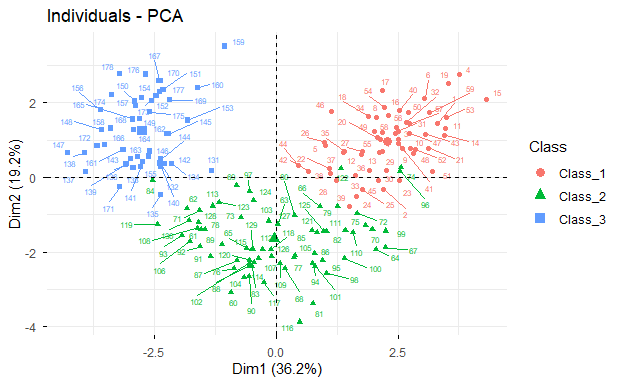
\includegraphics[width=0.7\textwidth]{Individuos_1_2_dim.png}
\caption{Gráfico de scores para las dimensiones 1 y 2}
\label{fig:scores12}
\end{figure}



En el primer gráfico de scores (Figura~\ref{fig:scores12}), se puede observar cómo, solamente con dos dimensiones, todos los individuos por clase se pueden ver bastante bien separados. Esto es un buen indicativo de cara al modelado y la predicción de sus clases. Se puede ver cómo la clase 2 puede encontrarse algo solapada con las clases 1 y 3, pero cómo estas dos últimas sí están completamente diferenciadas entre ellas.

\begin{figure}[H]
\centering
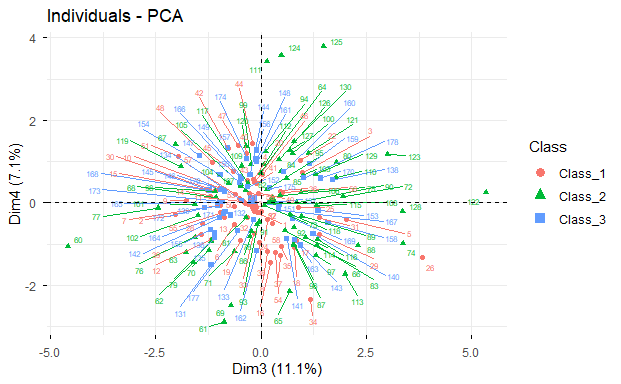
\includegraphics[width=0.7\textwidth]{Individuos_3_4_dim.png}
\caption{Gráfico de scores para las dimensiones 3 y 4}
\label{fig:scores34}
\end{figure}

Sin embargo, en la visualización de la tercera y cuarta dimensión (Figura~\ref{fig:scores34}) es complicado extraer conclusiones, ya que se observan todos los individuos entremezclados y no es posible distinguir una separación clara entre las clases.


% ─────────────────────────────────────────────────────────────────────────────
\section{Sesgos y limitaciones del dataset}

\subsection{Sesgos detectados}

\begin{description}[leftmargin=1.5cm, style=nextline]
    \item[Sesgo geogr\'afico.]
    Todos los vinos proceden de la misma regi\'on de Italia. El clasificador puede
    no generalizar a vinos de otras denominaciones de origen (p.ej., Rioja, Burdeos).

    \item[Sesgo temporal]
    El dataset no incluye el a\~no de cosecha. Las propiedades fisicoqu\'imicas
    var\'ian entre campa\~nas por factores clim\'aticos y de producci\'on, por lo que
    el modelo puede degradarse al aplicarse a vinos de cosechas muy diferentes.

    \item[Leve desbalanceo de clases.]
    La Clase~3 (27\%) est\'a subrepresentada respecto a la Clase~2 (40\%), lo que
    puede producir m\'etricas de \textit{accuracy} que deben ser revisadas.

    \item[Ausencia de variables sensoriales.]
    El dataset recoge \'unicamente propiedades fisicoqu\'imicas. La evaluaci\'on
    real del en\'ologo tambi\'en incorpora aspectos organol\'epticos (aroma, sabor,
    textura) no representados en los datos.
\end{description}

\subsection{Limitaciones para el modelado}

\begin{description}[leftmargin=1.5cm, style=nextline]
    \item[Small data (178 instancias).]
    El reducido tama\~no incrementa el riesgo de sobreajuste en modelos complejos.
    Se recomienda \textbf{validaci\'on cruzada} (k-fold con $k=10$).

    \item[Multicolinealidad entre variables fen\'olicas.]
    La alta correlaci\'on entre \texttt{TotalPhenols}, \texttt{Flavanoids} y
    \texttt{OD280/OD315} puede causar inestabilidad num\'erica en modelos como la
    regresi\'on log\'istica sin regularizaci\'on.

    \item[Escalas heterog\'eneas.]
    Requiere normalizaci\'on obligatoria antes de modelos basados en distancias
    (KNN, SVM) o en gradientes (redes neuronales, regresi\'on log\'istica).
\end{description}

% ─────────────────────────────────────────────────────────────────────────────
\section{Evaluaci\'on del rendimiento. M\'etricas}

\subsection{Formulaci\'on formal del problema}

El sistema VinOps debe aprender una funci\'on:
\[
    f\colon \mathbb{R}^{13} \rightarrow \{1,\,2,\,3\}
\]
tal que, dado un vector de caracter\'isticas fisicoqu\'imicas
$\mathbf{x} = (x_1,\, x_2,\, \ldots,\, x_{13})^{\top}$, el sistema prediga
correctamente la clase de cultivar $y \in \{1, 2, 3\}$.

Se trata de un \textbf{problema de clasificaci\'on multiclase supervisada} con 3
clases no ordenadas, lo que lo diferencia del problema de \textit{ranking} abordado
en el ejemplo HARP del profesor.

\subsection{M\'etricas de evaluaci\'on propuestas}

\begin{table}[H]
    \centering
    \caption{M\'etricas de evaluaci\'on propuestas para VinOps}
    \small
    \begin{tabular}{p{3cm} p{8.5cm}}
        \toprule
        \textbf{M\'etrica} & \textbf{Justificaci\'on} \\
        \midrule
        Macro F1-Score
            & Media no ponderada del F1 por clase. Penaliza por igual los errores
              en clases minoritarias. Recomendada para datasets con desbalanceo. \\[6pt]
        Accuracy
            & Proporci\'on de muestras correctamente clasificadas. \'Util como
              m\'etrica complementaria pero sensible al desbalanceo. \\[6pt]
        Balanced Accuracy
            & Media de la sensibilidad (recall) por clase. Robusta ante desbalanceo. \\[6pt]
        Matthews Correlation Coefficient
            & Coeficiente de correlaci\'on entre predicciones y etiquetas reales.
              Considera todas las celdas de la matriz de confusi\'on y es robusto
              ante desbalanceo. \\[6pt]
        Cohen's Kappa
            & Mide el acuerdo m\'as all\'a del azar. \'Util para comparar con HLP. \\
        \bottomrule
    \end{tabular}
    \label{tab:metricas}
\end{table}

\subsection{Rendimiento humano (HLP)}

Aunque no existe literatura espec\'ifica que cuantifique el rendimiento humano
(Human Level Performance) para este dataset, es razonable esperar que un
en\'ologo experto clasificando manualmente a partir de 13 valores fisicoqu\'imicos
obtenga una precisi\'on significativamente inferior (estimada entre
75\% y 85\%). Esta estimaci\'on se basa en la complejidad cognitiva de procesar simult\'aneamente
13 variables num\'ericas, frente a la capacidad
de los algoritmos para capturar patrones multivariantes complejos. 

La literatura cient\'ifica reporta que modelos de ML bien
entrenados alcanzan \textit{accuracy} del 98--99\% con t\'ecnicas como LDA
o SVM. El sistema VinOps deber\'ia superar claramente esta referencia humana.

\vspace{1mm}

\textit{Los valores anteriores sobre el rendimiento humano son orientativos y podrían variar 
en función del contexto real del proyecto y del perfil del equipo 
técnico contratado.}

\subsection{Benchmarks de referencia}

\begin{table}[H]
    \centering
        \caption{Benchmarks de referencia para el dataset Wine UCI
             \cite{UCIWine,Aeberhard1994,James2021,Hastie2009,Breiman2001,Cortes1995,Fisher1936}}
    \begin{tabular}{lcc}
        \toprule
        \textbf{Modelo} & \textbf{Accuracy aprox.} & \textbf{Observaciones} \\
        \midrule
        LDA (An\'alisis Discriminante Lineal) & $\approx 99\%$ & Alta interpretabilidad \\
        SVM (kernel RBF)                      & $\approx 98\%$ & Requiere normalizaci\'on \\
        Random Forest                         & $\approx 98\%$ & Robusto a outliers \\
        Regresi\'on Log\'istica (L2)          & $\approx 97\%$ & Requiere normalizaci\'on \\
        KNN ($k=3$)                           & $\approx 96\%$ & Requiere normalizaci\'on \\
        \'Arbol de decisi\'on                 & $\approx 92\%$ & Alta interpretabilidad \\
        \bottomrule
    \end{tabular}
    \label{tab:benchmarks}
\end{table}


\noindent Estos valores servir\'an como referencia para evaluar el rendimiento de los
modelos que se desarrollar\'an en el Hito~3. Un modelo que no supere los benchmarks
de la Tabla~\ref{tab:benchmarks} deber\'a ser revisado antes de proceder a las fases
de despliegue.

% ─────────────────────────────────────────────────────────────────────────────
\section{Justificaci\'on del dataset y decisiones tomadas}

A lo largo de este an\'alisis se han tomado las siguientes decisiones:

\begin{enumerate}
    \item \textbf{Uso del dataset Wine UCI sin modificaciones en este hito:} El
    dataset no presenta valores faltantes ni errores evidentes. La limpieza de
    outliers se abordar\'a en el Hito~3 (preprocesado).

    \item \textbf{Inclusi\'on de las 13 variables en el an\'alisis:} Aunque variables
    como \texttt{Ash} presentan bajo poder discriminante, se mantienen en el inventario
    para que la fase de selecci\'on de caracter\'isticas del Hito~3 determine
    formalmente cu\'ales deben eliminarse.

    \item \textbf{Selecci\'on del Macro F1-Score como m\'etrica principal:}
    Justificada por el desbalanceo moderado entre clases y por la necesidad de que el
    sistema funcione bien en todas las variedades vinc\'olas, incluyendo la menos
    representada (Clase~3).

    \item \textbf{No aplicaci\'on de pipelines de datos en este hito:} A diferencia
    del ejemplo HARP, el dataset Wine UCI no requiere la integraci\'on de m\'ultiples
    fuentes ni la transformaci\'on de datos brutos. Los datos ya est\'an estructurados
    en formato CSV, por lo que la construcci\'on de un pipeline complejo no aporta
    valor en esta fase.
\end{enumerate}

